\chapter{Cambios de estado de un cuerpo puro}\label{ch:b1:phase-changes}

El agua es la única sustancia que todo el mundo ha visto en los tres
estados, y es el fluido de trabajo de casi todas las centrales
eléctricas del mundo, el \omterm{def:b1:heat-engines:vapourcycle}{refrigerante} de las primeras máquinas de hielo
y el motor del tiempo atmosférico. El hielo se funde a una temperatura
que no se mueve mientras el calor entra a raudales; un hervidor hierve a
\qty{100}{\degreeCelsius} a orillas del mar y a \qty{70}{\degreeCelsius}
en el Everest; una botella cerrada de agua muy fría se congela entera de
un golpecito. Este capítulo traza el mapa de las \omterm{def:b1:phase-changes:phase}{fases} de un \omterm{def:b1:phase-changes:phase}{cuerpo puro}
--- los diagramas $(T, P)$ y $(v, P)$ --- y da las tres herramientas que
lo acompañan: la \omterm{thm:b1:phase-changes:lever}{regla de la palanca} (cuánto hay de cada \omterm{def:b1:phase-changes:phase}{fase}), el \omterm{def:b1:phase-changes:phase}{calor
latente} (lo que cuesta un cambio, en energía y en entropía) y la
\omterm{thm:b1:phase-changes:clapeyron}{relación de Clausius--Clapeyron} (la pendiente de las líneas frontera).
Acaba donde el mapa falla: en los \omterm{def:b1:phase-changes:metastable}{estados metaestables}, de donde vienen
el tiempo atmosférico y las sorpresas de la olla a presión.

\section{Las fases y el diagrama $(T, P)$}

\begin{definition}[Cuerpo puro, fase, cambio de estado]\label{def:b1:phase-changes:phase}
\index{fase}\index{cambio de estado}\index{cuerpo puro}\index{calor latente}
Un \emph{cuerpo puro} es un cuerpo formado por una sola especie química.
Una \emph{fase} es una parte de él homogénea en sus propiedades físicas:
sólido, líquido, gas (\emph{vapor} cuando coexiste con su líquido). Un
\emph{cambio de estado} (fusión/solidificación, vaporización/
licuefacción, sublimación/condensación sólida) es el paso de una fase a
otra; a presión fija ocurre a temperatura fija, con intercambio de calor
pero sin variación de temperatura: el \emph{calor latente}.
\end{definition}

\begin{proposition}[Diagrama de equilibrio]\label{prop:b1:phase-changes:PTdiagram}
\index{diagrama de fases}\index{punto triple}\index{punto crítico}\index{presión de vapor saturante}
En el plano $(T, P)$ cada \omterm{def:b1:phase-changes:phase}{fase} ocupa una región; dos \omterm{def:b1:phase-changes:phase}{fases} coexisten solo
a lo largo de una curva (sublimación, fusión, vaporización), y las tres
solo en un punto, el \emph{\omterm{prop:b1:phase-changes:PTdiagram}{punto triple}}. La curva de vaporización
$P = P_s(T)$ --- la \emph{\omterm{prop:b1:phase-changes:PTdiagram}{presión de vapor saturante}} --- acaba en el
\emph{\omterm{prop:b1:phase-changes:PTdiagram}{punto crítico}} $(T_c, P_c)$, más allá del cual líquido y gas dejan
de distinguirse. Para el agua: \omterm{prop:b1:phase-changes:PTdiagram}{punto triple} \qty{273.16}{K}, \qty{611}{Pa};
\omterm{prop:b1:phase-changes:PTdiagram}{punto crítico} \qty{647}{K}, \qty{221}{bar}. La curva de fusión del agua
se inclina hacia la izquierda (el hielo es menos denso que el agua); en
casi todas las demás sustancias se inclina hacia la derecha.
\end{proposition}
\admitted

\begin{omfigure}
\begin{tikzpicture}[font=\small, x=1cm, y=1cm, >=Stealth]
  \draw[->] (0,0) -- (8.4,0) node[below] {$T$};
  \draw[->] (0,0) -- (0,5.2) node[left] {$P$};
  \coordinate (Tp) at (2.4,1.2);
  \coordinate (C) at (6.8,4.4);
  \draw[omDef, very thick] (0.3,0.08) .. controls (1.4,0.3) .. (Tp);
  \draw[omThm, very thick] (Tp) .. controls (2.2,2.8) .. (1.9,5.0);
  \draw[omProp, very thick] (Tp) .. controls (4.6,1.6) and (6.0,3.0) .. (C);
  \fill (Tp) circle (2pt) node[below right, font=\footnotesize] {punto triple $\mathrm T$};
  \fill (C) circle (2pt) node[above left, font=\footnotesize] {punto crítico $\mathrm C$};
  \node at (0.9,3.4) {sólido};
  \node at (3.6,4.0) {líquido};
  \node at (6.6,0.9) {gas};
  \node[omDef, font=\footnotesize, anchor=north] at (1.3,0.9) {sublimación};
  \node[omThm, font=\footnotesize, rotate=80] at (1.8,3.3) {fusión};
  \node[omProp, font=\footnotesize, rotate=35] at (5.35,1.9) {vaporización};
  \draw[dashed] (0,2.4) node[left, font=\footnotesize] {\qty{1}{atm}} -- (8.0,2.4);
  \fill (2.25,2.4) circle (1.6pt) node[above left, font=\footnotesize, xshift=2pt] {\qty{0}{\degreeCelsius}};
  \fill (5.12,2.42) circle (1.6pt) node[above left, font=\footnotesize] {\qty{100}{\degreeCelsius}};
  \draw[dotted] (C) -- (6.8,0) node[below, font=\footnotesize] {$T_c$};
  \node[font=\footnotesize, align=center] at (7.6,3.3) {fluido\\ supercrítico};
\end{tikzpicture}

{\small El \omterm{prop:b1:phase-changes:PTdiagram}{diagrama de fases} del agua (no está a escala). Calentar a
presión atmosférica sigue la isobara de trazos: el hielo se funde donde
esta corta a la curva de fusión y el agua hierve donde corta a la de
vaporización. La curva de fusión del agua se inclina hacia la izquierda:
la presión rebaja su punto de fusión.}
\end{omfigure}

\begin{remark}[Ebullición, evaporación y la olla a presión]\label{rem:b1:phase-changes:boiling}
Un líquido se \emph{evapora} a cualquier temperatura desde su superficie,
mientras la presión parcial de su vapor por encima esté por debajo de
$P_s(T)$; \emph{hierve} cuando $P_s(T)$ alcanza la presión ambiente, de
modo que pueden crecer burbujas de vapor en su interior. El agua hierve a
\qty{100}{\degreeCelsius} porque
$P_s(\qty{100}{\degreeCelsius}) = \qty{1.013}{bar}$; a
\qty{0.33}{bar} en el Everest hierve cerca de \qty{70}{\degreeCelsius}, y
en una olla a presión a \qty{1.8}{bar}, cerca de \qty{117}{\degreeCelsius}.
La temperatura de un líquido en ebullición la clava la presión --- hecho
que sirvió durante dos siglos para definir la escala Celsius.
\end{remark}

\section{El diagrama $(v, P)$ y la regla de la palanca}

\begin{proposition}[Isotermas de Andrews]\label{prop:b1:phase-changes:andrews}
\index{isotermas de Andrews}\index{curva de saturación}
En el plano de Clapeyron $(v, P)$ del volumen másico, una isoterma
$T < T_c$ tiene tres partes: una rama muy empinada (líquido, casi
incompresible), un \emph{escalón} horizontal a $P = P_s(T)$ donde coexisten
líquido y vapor, y una rama parecida a una hipérbola (vapor). Los
extremos del escalón son los volúmenes másicos $v_l(T)$ y $v_v(T)$ del
líquido y del vapor saturantes; su lugar geométrico es la \emph{\omterm{prop:b1:phase-changes:andrews}{curva de
saturación}} (la campana), cuya cima es el \omterm{prop:b1:phase-changes:PTdiagram}{punto crítico}, donde la
isoterma $T_c$ tiene una inflexión horizontal. Por encima de $T_c$ no hay
escalón.
\end{proposition}
\admitted

\begin{theorem}[Regla de la palanca]\label{thm:b1:phase-changes:lever}
\index{regla de la palanca}\index{título (fracción másica de vapor)}
Una masa $m$ de volumen másico $v$ situada en el escalón a $T$ se reparte
en una fracción másica de vapor $x = m_v/m$ (el \emph{título}) y una
fracción líquida $1 - x$, con
\[
v = (1 - x)v_l + x\,v_v , \qquad\text{es decir}\qquad
x = \frac{v - v_l}{v_v - v_l} = \frac{LM}{LV} ,
\]
la razón de los segmentos que el punto de estado $M$ recorta en el
escalón. La misma regla vale para toda magnitud extensiva por unidad de
masa ($u$, $h$, $s$): $h = (1 - x)h_l + xh_v$.
\end{theorem}

\begin{proof}
Los volúmenes se suman: $V = m_lv_l + m_vv_v$; divídase por $m$. La
energía, la \omterm{def:b1:first-law:enthalpy}{entalpía} y la entropía son también extensivas.
\end{proof}

\begin{omfigure}
\begin{tikzpicture}[font=\small, x=1cm, y=1cm, >=Stealth]
  \draw[->] (0,0) -- (9.4,0) node[below] {$v$};
  \draw[->] (0,0) -- (0,5.4) node[left] {$P$};
  % dome
  \draw[omDef, thick] plot[smooth, tension=0.8] coordinates {(0.7,0.2) (0.8,2.0) (1.3,3.6) (2.6,4.5) (4.0,3.5) (5.2,2.0) (7.0,1.1) (9.0,0.5)};
  \fill (2.6,4.5) circle (2pt) node[above, font=\footnotesize] {$\mathrm C$};
  % isotherm T1 < Tc
  \draw[omProp, thick] (0.62,5.0) .. controls (0.7,3.2) .. (0.8,2.0) -- (5.2,2.0)
        .. controls (6.4,1.6) and (7.6,1.1) .. (9.2,0.85);
  \node[omProp, font=\footnotesize, anchor=west] at (9.0,1.2) {$T_1$};
  % critical isotherm
  \draw[omThm, thick] (1.1,5.3) .. controls (1.8,4.6) and (2.2,4.5) .. (2.6,4.5)
        .. controls (3.6,4.5) and (5.0,3.4) .. (9.2,2.4);
  \node[omThm, font=\footnotesize, anchor=west] at (9.0,2.7) {$T_c$};
  % supercritical isotherm
  \draw[omExo, thick] (1.7,5.4) .. controls (2.6,4.9) and (4.0,4.4) .. (9.2,3.6);
  \node[omExo, font=\footnotesize, anchor=west] at (9.0,3.9) {$T_2 > T_c$};
  % lever
  \fill (0.8,2.0) circle (1.6pt) node[above left, font=\footnotesize] {$L$};
  \fill (5.2,2.0) circle (1.6pt) node[above right, font=\footnotesize] {$V$};
  \fill (2.5,2.0) circle (1.6pt) node[above, font=\footnotesize] {$M$};
  \draw[<->, omDef] (0.8,1.55) -- (2.5,1.55) node[midway, below, font=\footnotesize] {$x\,(v_v - v_l)$};
  \draw[<->, omDef] (2.5,1.55) -- (5.2,1.55) node[midway, below, font=\footnotesize] {$(1 - x)(v_v - v_l)$};
  \draw[dashed] (0.8,2.0) -- (0.8,0) node[below, font=\footnotesize] {$v_l$};
  \draw[dashed] (5.2,2.0) -- (5.2,0) node[below, font=\footnotesize] {$v_v$};
  \draw[dashed] (2.5,2.0) -- (2.5,0) node[below, font=\footnotesize] {$v$};
  \node[font=\footnotesize, rotate=90] at (0.3,3.4) {líquido};
  \node[font=\footnotesize] at (3.7,0.6) {líquido + vapor};
  \node[font=\footnotesize] at (7.6,0.25) {vapor};
  \draw[dashed] (0,2.0) node[left, font=\footnotesize] {$P_s(T_1)$} -- (0.8,2.0);
\end{tikzpicture}

{\small \omterm{prop:b1:phase-changes:andrews}{Isotermas de Andrews} en el diagrama de Clapeyron. Bajo la
campana, la isoterma $T_1$ es un escalón a $P_s(T_1)$; un estado $M$
sobre él es una mezcla cuya fracción de vapor $x$ es la razón $LM/LV$. La
isoterma crítica toca la campana en su cima con una inflexión
horizontal; por encima de $T_c$ no hay escalón ni distinción entre
líquido y gas.}
\end{omfigure}

\begin{example}[Un hervidor y una caldera]\label{ex:b1:phase-changes:lever}
Agua a \qty{100}{\degreeCelsius} y \qty{1}{atm}: $v_l = \qty{1.04e-3}{m^3/kg}$,
$v_v = \qty{1.67}{m^3/kg}$ --- una razón de $1600$. Un recipiente cerrado
de \qty{1.0}{L} que contiene \qty{0.50}{kg} de agua a esa temperatura tiene $v =
\qty{2.0e-3}{m^3/kg}$ y $x = (2.0 - 1.04) \times 10^{-3}/1.67 = 5.8 \times 10^{-4}$:
\qty{0.29}{g} de vapor ocupan la mitad del recipiente. Duplicar la masa
de vapor en un recipiente cerrado apenas mueve el punto de estado; la
presión la fija la temperatura por sí sola.
\end{example}

\section{Energética de un cambio de estado}

\begin{proposition}[Calor latente, entalpía y entropía de transición]\label{prop:b1:phase-changes:latent}
\index{entalpía de transición}\index{entropía de transición}
A la temperatura $T$ y la presión $P_s(T)$ de coexistencia, la transición
de la unidad de masa de la \omterm{def:b1:phase-changes:phase}{fase} 1 a la \omterm{def:b1:phase-changes:phase}{fase} 2 es reversible, isoterma e
isobara, y
\[
L_{12}(T) = h_2 - h_1 , \qquad s_2 - s_1 = \frac{L_{12}}{T} , \qquad
u_2 - u_1 = L_{12} - P_s(v_2 - v_1) .
\]
$L_{12} > 0$ cuando se va hacia la \omterm{def:b1:phase-changes:phase}{fase} menos ordenada (fusión,
vaporización, sublimación), y $L_{21} = -L_{12}$. Para el agua a \qty{1}{atm}:
$L_f = \qty{334}{kJ/kg}$ a \qty{0}{\degreeCelsius} y $L_v = \qty{2257}{kJ/kg}$ a
\qty{100}{\degreeCelsius}.
\end{proposition}

\begin{proof}
A presión constante, el calor recibido es $\Delta H$
(\cref{prop:b1:first-law:qvqp}); reversible e isotermo, vale
$T\Delta S$ (\cref{prop:b1:second-law-entropy:identity}); y $U = H - PV$.
\end{proof}

\begin{example}[Adónde va el calor de vaporización]\label{ex:b1:phase-changes:whereheat}
Para el agua a \qty{100}{\degreeCelsius}: $P_s(v_v - v_l) = 1.013 \times 10^5 \times
1.67 = \qty{169}{kJ/kg}$, luego $u_v - u_l = 2257 - 169 = \qty{2088}{kJ/kg}$:
el $93\%$ del \omterm{def:b1:phase-changes:phase}{calor latente} se emplea en separar las moléculas y el $7\%$
en apartar la atmósfera. La entropía de vaporización,
$2257/373 = \qty{6.05}{kJ/(kg.K)}$, aplasta a la de fusión, $334/273 =
\qty{1.22}{kJ/(kg.K)}$: fundir afloja las moléculas, hervir las libera.
\end{example}

\begin{method}[Calorimetría con cambios de estado]\label{meth:b1:phase-changes:calorimetry}
En un recipiente aislado a presión constante, $\sum\Delta H_i = 0$.
Supóngase el estado final (qué \omterm{def:b1:phase-changes:phase}{fases} hay presentes y a qué temperatura);
escríbase el $\Delta H$ de cada cuerpo como calores sensibles $mc\,\Delta T$
más \omterm{def:b1:phase-changes:phase}{calores latentes} $\pm mL$ por los cambios que sufra; resuélvase, y
\emph{compruébese la suposición}: un cuerpo que acabe por encima de su
temperatura de ebullición o por debajo de la de fusión, o una masa
negativa de una \omterm{def:b1:phase-changes:phase}{fase}, significan que la suposición era falsa --- el
estado final es entonces una mezcla a la temperatura de transición, y la
incógnita pasa a ser la masa transformada (\cref{ex:b1:first-law:ice}).
\end{method}

\begin{example}[El vapor quema]\label{ex:b1:phase-changes:steam}
\qty{10}{g} de vapor a \qty{100}{\degreeCelsius} que se condensan sobre la
piel entregan $0.010 \times 2257 = \qty{22.6}{kJ}$ antes de haberse enfriado
un solo grado --- tanto como los que \qty{10}{g} de agua hirviendo dan al
enfriarse \qty{540}{K}. Por eso escalda el vapor mucho más que el agua a
la misma temperatura, y por eso un radiador de vapor necesita tan poco caudal.
\end{example}

\begin{omfigure}
\begin{tikzpicture}[font=\small, x=1cm, y=1cm, >=Stealth]
  \draw[->] (0,0) -- (9.0,0) node[below] {$s$};
  \draw[->] (0,0) -- (0,5.2) node[left] {$T$};
  \draw[omDef, thick] (0.9,0.3) .. controls (1.3,2.6) and (2.6,4.4) .. (4.0,4.6)
        .. controls (5.4,4.4) and (7.0,2.4) .. (8.4,0.3);
  \fill (4.0,4.6) circle (2pt) node[above, font=\footnotesize] {$\mathrm C$};
  % isobar at T1
  \draw[omProp, thick] (0.6,0.35) .. controls (1.1,1.2) .. (1.65,2.6) -- (6.65,2.6)
        .. controls (7.4,3.0) and (8.0,3.6) .. (8.6,4.5);
  \node[omProp, font=\footnotesize, anchor=west] at (8.6,4.6) {isobara $P_1$};
  \draw[dashed] (1.65,2.6) -- (1.65,0) node[below, font=\footnotesize] {$s_l$};
  \draw[dashed] (6.65,2.6) -- (6.65,0) node[below, font=\footnotesize] {$s_v$};
  \draw[dashed] (0,2.6) node[left, font=\footnotesize] {$T_1$} -- (1.65,2.6);
  \draw[<->, omThm] (1.65,2.9) -- (6.65,2.9) node[midway, above, font=\footnotesize] {$s_v - s_l = L_v/T_1$};
  \fill[omThm!15] (1.65,0) rectangle (6.65,2.6);
  \node[font=\footnotesize, omThm] at (4.15,1.2) {área $= L_v$};
  \node[font=\footnotesize] at (1.0,3.9) {líquido};
  \node[font=\footnotesize] at (8.3,1.9) {vapor};
  \node[font=\footnotesize] at (4.15,2.0) {líquido + vapor};
\end{tikzpicture}

{\small La misma campana en el \omterm{def:b1:second-law-entropy:TS}{diagrama entrópico}. Una isobara la
atraviesa como un segmento horizontal de longitud $L_v/T$; el área bajo
el segmento es el \omterm{def:b1:phase-changes:phase}{calor latente}. Los ciclos de las centrales eléctricas
se dibujan en este plano, y el título a la salida de la turbina se lee
sobre el segmento con la \omterm{thm:b1:phase-changes:lever}{regla de la palanca}.}
\end{omfigure}

\section{La relación de Clausius--Clapeyron}

\begin{theorem}[Clausius--Clapeyron]\label{thm:b1:phase-changes:clapeyron}
\index{relación de Clausius--Clapeyron}
A lo largo de una curva de coexistencia de las \omterm{def:b1:phase-changes:phase}{fases} 1 y 2,
\[
\frac{\dd P_s}{\dd T} = \frac{L_{12}(T)}{T\,(v_2 - v_1)} .
\]
\end{theorem}

\begin{proof}
Hágase recorrer a la unidad de masa un \omterm{def:b1:heat-engines:carnotcycle}{ciclo de Carnot} infinitesimal
dentro de la campana: transición completa $1 \to 2$ por el escalón a
$T + \dd T$ y presión $P_s + \dd P_s$ (calor recibido $L_{12}$ a primer
orden); un paso adiabático infinitesimal hasta $T$; la transición inversa
por el escalón a $T$, $P_s$; un paso adiabático de vuelta. El ciclo es
reversible y ditérmico entre $T + \dd T$ y $T$, luego su \omterm{def:b1:heat-engines:efficiency}{rendimiento} vale
$\dd T/T$ (\cref{thm:b1:heat-engines:carnot}); su trabajo, el área del
rectángulo delgado, vale $\dd P_s\,(v_2 - v_1)$. De ahí $\dd P_s\,(v_2 - v_1)/L_{12} =
\dd T/T$.
\end{proof}

\begin{omfigure}
\begin{tikzpicture}[font=\small, x=1cm, y=1cm, >=Stealth]
  \draw[->] (0,0) -- (8.6,0) node[below] {$v$};
  \draw[->] (0,0) -- (0,4.6) node[left] {$P$};
  \draw[omDef, thick] (0.6,0.2) .. controls (0.75,2.0) and (1.6,3.7) .. (2.6,4.0)
        .. controls (3.6,3.7) and (5.8,1.6) .. (8.2,0.4);
  \fill[omProp!25] (0.92,2.0) -- (4.88,2.0) -- (4.95,2.3) -- (0.9,2.3) -- cycle;
  \draw[omProp, thick] (0.92,2.0) -- (4.88,2.0) node[pos=0.5, below, font=\footnotesize] {$T$, $P_s$};
  \draw[omThm, thick] (0.9,2.3) -- (4.95,2.3) node[pos=0.5, above, font=\footnotesize] {$T + \dd T$, $P_s + \dd P_s$};
  \draw[<->] (6.2,2.0) -- (6.2,2.3) node[midway, right, font=\footnotesize] {$\dd P_s$};
  \draw[dotted] (4.88,2.0) -- (6.3,2.0); \draw[dotted] (4.95,2.3) -- (6.3,2.3);
  \draw[<->] (0.92,1.4) -- (4.88,1.4) node[midway, below, font=\footnotesize] {$v_2 - v_1$};
  \draw[dotted] (0.92,2.0) -- (0.92,1.3); \draw[dotted] (4.88,2.0) -- (4.88,1.3);
  \node[font=\footnotesize, omProp, anchor=west] at (4.0,3.5) {$-W = \dd P_s\,(v_2 - v_1)$, \; $Q_h = L_{12}$};
\end{tikzpicture}

{\small El \omterm{def:b1:heat-engines:carnotcycle}{ciclo de Carnot} infinitesimal que demuestra la \omterm{thm:b1:phase-changes:clapeyron}{relación de
Clausius--Clapeyron}: dos escalones separados por $\dd T$, unidos por
pasos adiabáticos demasiado cortos para dibujarlos; el \omterm{thm:b1:heat-engines:carnot}{teorema de Carnot}
iguala a $\dd T/T$ la razón entre su área y el calor recibido.}
\end{omfigure}

\begin{corollary}[Presión de vapor saturante de un líquido]\label{cor:b1:phase-changes:vapourpressure}
Si el vapor es un \omterm{def:b1:kinetic-theory:model}{gas perfecto} y $v_v \gg v_l$, de modo que $v_v - v_l \approx
RT/(MP_s)$, y si $L_v$ varía poco,
\[
\frac{\dd P_s}{P_s} = \frac{ML_v}{R}\,\frac{\dd T}{T^2} , \qquad
\ln\frac{P_s(T)}{P_s(T_0)} = \frac{ML_v}{R}\Bigl(\frac{1}{T_0} - \frac{1}{T}\Bigr) :
\]
la presión de vapor crece aproximadamente de forma exponencial con la
temperatura. Para el agua cerca de \qty{100}{\degreeCelsius}, $ML_v/R = 0.018 \times 2.257 \times 10^6/
8.314 = \qty{4890}{K}$ y $\dd P_s/\dd T = 2.257 \times 10^6/(373 \times 1.67) =
\qty{3.6}{kPa/K}$: cada \omterm{def:b1:kinetic-theory:temperature}{kelvin} de más en la temperatura de ebullición
cuesta \qty{36}{mbar} de presión.
\end{corollary}

\begin{proof}
Sustitúyase $v_v - v_l \approx RT/(MP_s)$ en el teorema y sepárense las
variables; intégrese con $L_v$ constante.
\end{proof}

\begin{omfigure}
\begin{tikzpicture}
\begin{axis}[omaxis, axis x line=bottom, axis y line=left, width=10.5cm, height=6.2cm,
    xlabel={$T$ (\unit{\degreeCelsius})}, ylabel={$P_s$ (\unit{kPa})},
    xlabel style={at={(axis description cs:0.5,-0.14)}, anchor=north},
    xmin=0, xmax=130, ymin=0, ymax=230, xtick={0,20,...,120}, ytick={50,100,150,200}, samples=120, clip=false]
  \addplot[omDef, thick, domain=0:125] {0.133322*10^(8.07131-1730.63/(233.426+x))};
  \addplot[black, dashed] coordinates {(0,101.3) (100,101.3) (100,0)};
  \addplot[black, dashed] coordinates {(0,33) (71,33) (71,0)};
  \addplot[black, dashed] coordinates {(0,180) (117,180) (117,0)};
  \node[font=\footnotesize, anchor=south west] at (axis cs:2,103) {nivel del mar: \qty{100}{\degreeCelsius}};
  \node[font=\footnotesize, anchor=south west] at (axis cs:2,35) {Everest (\qty{0.33}{bar}): \qty{71}{\degreeCelsius}};
  \node[font=\footnotesize, anchor=south west] at (axis cs:2,182) {olla a presión (\qty{1.8}{bar}): \qty{117}{\degreeCelsius}};
\end{axis}
\end{tikzpicture}

{\small La \omterm{prop:b1:phase-changes:PTdiagram}{presión de vapor saturante} del agua. La curva es casi una
exponencial en $-1/T$; la temperatura de ebullición es aquella a la que
corta a la presión ambiente.}
\end{omfigure}

\begin{example}[El hielo bajo un patín]\label{ex:b1:phase-changes:skate}
Para el equilibrio hielo--agua, $L_f = \qty{334}{kJ/kg}$ y $v_l - v_s = (1.000 - 1.091)
\times 10^{-3} = \qty{-9.1e-5}{m^3/kg}$: $\dd P/\dd T = 3.34 \times 10^5/(273 \times
(-9.1 \times 10^{-5})) = \qty{-1.3e7}{Pa/K} = \qty{-130}{bar/K}$. Un patinador
de \qty{70}{kg} sobre una cuchilla de \qty{30}{cm} por \qty{3}{mm} ($\qty{9}{cm^2}$) ejerce
unos \qty{8}{bar}, que rebajan el punto de fusión en \qty{0.06}{K} --- la fusión por presión no es la razón de que los patines deslicen (una fina
capa superficial del hielo se comporta ya por sí sola como un líquido, y
el rozamiento calienta); pero la pendiente negativa es real, y es la
razón de que un alambre cargado con pesas corte un bloque de hielo que
vuelve a congelarse detrás de él.
\end{example}

\section{Los estados metaestables}

\begin{definition}[Sobrefusión, sobrecalentamiento]\label{def:b1:phase-changes:metastable}
\index{sobrefusión}\index{sobrecalentamiento}\index{estado metaestable}\index{nucleación}
Una \omterm{def:b1:phase-changes:phase}{fase} puede persistir más allá de su frontera de equilibrio: agua
líquida enfriada por debajo de \qty{0}{\degreeCelsius} sin congelarse (la
\emph{sobrefusión}), calentada por encima de su temperatura de ebullición
sin hervir (el \emph{sobrecalentamiento}), vapor comprimido más allá de
$P_s$ sin condensar (la sobresaturación). Estos \emph{estados
metaestables} exigen la ausencia de puntos de \emph{nucleación} --- polvo,
arañazos, gas disuelto, cristales de hielo --- sobre los que pueda
arrancar la nueva \omterm{def:b1:phase-changes:phase}{fase}; una perturbación los vuelca de golpe, y de modo
irreversible, hacia el equilibrio.
\end{definition}

\begin{example}[La botella en sobrefusión]\label{ex:b1:phase-changes:supercooled}
Agua en reposo a \qty{-8}{\degreeCelsius} en una botella limpia, y un
golpe: los cristales de hielo la recorren como un disparo y la
temperatura salta a \qty{0}{\degreeCelsius}. El proceso es adiabático y
rápido, de modo que el calor sensible $c\,\Delta T$ congela una fracción $x = c\,\Delta T/L_f = 4.18 \times 8/334 =
0.10$ del agua; la entropía creada, $c\ln(273/265) - xL_f/273 =
124 - 122 = \qty{+2}{J/(kg.K)}$, es positiva como ha de ser. Las nubes
están llenas de gotitas en \omterm{def:b1:phase-changes:metastable}{sobrefusión} hasta \qty{-40}{\degreeCelsius}; el
engelamiento de los aviones y la siembra de nubes explotan ambos ese hecho.
\end{example}

\begin{remark}[Perlas de ebullición y cámaras de burbujas]\label{rem:b1:phase-changes:nucleation}
Una burbuja de radio $r$ en un líquido a la presión $P$ contiene vapor a
$P + 2\sigma/r$ (tensión superficial $\sigma$, volumen del Año 2); solo
puede crecer si $P_s(T) > P + 2\sigma/r$, de modo que un líquido limpio en
su temperatura de ebullición no tiene ninguna burbuja lo bastante pequeña
para arrancar y se sobrecalienta varios \omterm{def:b1:kinetic-theory:temperature}{kelvin} antes de estallar --- los
``sobresaltos'' que evitan las perlas de ebullición ofreciendo cavidades
llenas de gas atrapado. La cámara de burbujas de la física de partículas
funcionaba con la misma inestabilidad al revés: un líquido
sobrecalentado hierve primero a lo largo de la traza de una partícula ionizante.
\end{remark}

\begin{example}[Humedad y rocío]\label{ex:b1:phase-changes:dew}
\index{humedad relativa}\index{punto de rocío}
El aire contiene vapor de agua a una presión parcial $P_v \leq P_s(T)$; la
\emph{\omterm{ex:b1:phase-changes:dew}{humedad relativa}} es $P_v/P_s(T)$, y el \emph{\omterm{ex:b1:phase-changes:dew}{punto de rocío}}, la
temperatura a la que $P_s$ baja hasta $P_v$. Aire a \qty{25}{\degreeCelsius}
($P_s = \qty{3.17}{kPa}$) con un $60\%$ de humedad tiene $P_v = \qty{1.9}{kPa}$
y $\rho_v = P_vM/(RT) = \qty{14}{g/m^3}$, y deja rocío sobre cualquier
superficie por debajo de unos \qty{17}{\degreeCelsius} --- la hierba al
alba, la botella fría, el espejo del baño. Si asciende, ese mismo aire se
enfría adiabáticamente a \qty{9.8}{K/km} (\cref{pb:b1:phase-changes:1}) y
alcanza su \omterm{ex:b1:phase-changes:dew}{punto de rocío} hacia un kilómetro de altura: ahí está la base
plana de los cúmulos.
\end{example}

\section{Ejercicios}

\begin{exercise}[$\star$]\label{exo:b1:phase-changes:1}
Con el diagrama del curso, dese la \omterm{def:b1:phase-changes:phase}{fase} del agua (a) a
\qty{20}{\degreeCelsius} bajo \qty{0.5}{kPa}; (b) a \qty{-5}{\degreeCelsius}
bajo \qty{1}{bar}; (c) a \qty{400}{\degreeCelsius} bajo \qty{200}{bar};
(d) a \qty{0.01}{\degreeCelsius} bajo \qty{611}{Pa}. ¿Por qué se seca un
charco a \qty{20}{\degreeCelsius} si el agua ``hierve a 100''?
\end{exercise}

\begin{exercise}[$\star$]\label{exo:b1:phase-changes:2}
Se burbujean \qty{100}{g} de vapor a \qty{100}{\degreeCelsius} en
\qty{1.0}{kg} de agua a \qty{20}{\degreeCelsius} en un recipiente aislado.
Temperatura final ($L_v = \qty{2257}{kJ/kg}$, $c = \qty{4.18}{kJ/(kg.K)}$).
Compárese con añadir \qty{100}{g} de agua a \qty{100}{\degreeCelsius}.
\end{exercise}

\begin{exercise}[$\star$]\label{exo:b1:phase-changes:3}
Un recipiente rígido de \qty{2.0}{L} contiene \qty{1.0}{kg} de agua a
\qty{150}{\degreeCelsius} en equilibrio líquido--vapor ($P_s =
\qty{4.76}{bar}$, $v_l = \qty{1.09e-3}{m^3/kg}$, $v_v = \qty{0.393}{m^3/kg}$).
Título, masa de vapor y volumen ocupado por el líquido.
\end{exercise}

\begin{exercise}[$\star$]\label{exo:b1:phase-changes:4}
Entropía de vaporización del agua a \qty{100}{\degreeCelsius}, por
kilogramo y por \omterm{def:b1:kinetic-theory:scales}{mol}; entropía de fusión por \omterm{def:b1:kinetic-theory:scales}{mol} a \qty{0}{\degreeCelsius}.
Muchos líquidos corrientes tienen una entropía molar de vaporización
próxima a \qty{88}{J/(\omterm{def:b1:kinetic-theory:scales}{mol}.K)} (regla de Trouton): ¿es corriente el agua?
\end{exercise}

\begin{exercise}[$\star\star$]\label{exo:b1:phase-changes:5}
Temperatura de ebullición del agua en la cima del Everest, $P =
\qty{0.33}{bar}$, a partir de \cref{cor:b1:phase-changes:vapourpressure} con
$ML_v/R = \qty{4890}{K}$; y a \qty{2000}{m} ($P = \qty{0.80}{bar}$). ¿En qué
queda un huevo de \qty{3}{min}?
\end{exercise}

\begin{exercise}[$\star\star$]\label{exo:b1:phase-changes:6}
Temperatura dentro de una olla a presión cuya válvula abre a \qty{1.8}{bar}
absolutos; y la misma si la válvula estuviera tarada a \qty{2.5}{bar}. El
vapor a \qty{1.8}{bar} tiene $v_v = \qty{0.98}{m^3/kg}$: ¿cuántos gramos de
vapor contiene una olla de \qty{6}{L} sobre \qty{4}{L} de agua?
\end{exercise}

\begin{exercise}[$\star\star$]\label{exo:b1:phase-changes:7}
Pendiente de la curva de fusión del agua a \qty{0}{\degreeCelsius} ($L_f =
\qty{334}{kJ/kg}$, $v_s = \qty{1.091e-3}{m^3/kg}$, $v_l = \qty{1.000e-3}{m^3/kg}$).
¿A qué presión se funde el hielo a \qty{-1}{\degreeCelsius}? Hielo en el
fondo de un casquete de \qty{3}{km} ($\rho = \qty{917}{kg/m^3}$):
temperatura de fusión allí y una consecuencia para el flujo de los glaciares.
\end{exercise}

\begin{exercise}[$\star\star$]\label{exo:b1:phase-changes:8}
Un kilogramo de agua se evapora por completo a \qty{100}{\degreeCelsius} bajo
\qty{1}{atm} ($v_v = \qty{1.673}{m^3/kg}$, $v_l = \qty{1.04e-3}{m^3/kg}$).
Trabajo recibido, calor recibido, $\Delta U$, $\Delta H$ y $\Delta S$ del
agua; entropía creada si el calor viene de una llama a
\qty{1500}{K}.
\end{exercise}

\begin{exercise}[$\star\star$]\label{exo:b1:phase-changes:9}
Presiones de saturación: \qty{1.23}{kPa} (\qty{10}{\degreeCelsius}), \qty{1.70}{kPa}
(\qty{15}{\degreeCelsius}), \qty{2.34}{kPa} (\qty{20}{\degreeCelsius}), \qty{3.17}{kPa}
(\qty{25}{\degreeCelsius}), \qty{4.24}{kPa} (\qty{30}{\degreeCelsius}). Una
habitación a \qty{22}{\degreeCelsius} tiene una \omterm{ex:b1:phase-changes:dew}{humedad relativa} del $70\%$:
presión de vapor, \omterm{ex:b1:phase-changes:dew}{punto de rocío} (interpólese) y masa de vapor de agua en
\qty{50}{m^3}. Un cristal de ventana a \qty{12}{\degreeCelsius}: ¿se empaña?
Si se calienta la habitación a \qty{25}{\degreeCelsius} sin añadir agua:
nueva humedad.
\end{exercise}

\begin{exercise}[$\star\star\star$]\label{exo:b1:phase-changes:10}
\emph{El \omterm{prop:b1:phase-changes:PTdiagram}{punto triple}.} (a) Muéstrese, por el carácter de función de
estado de $h$, que en el \omterm{prop:b1:phase-changes:PTdiagram}{punto triple} $L_s = L_f + L_v$ (sublimación =
fusión + vaporización). (b) Muéstrese con Clausius--Clapeyron que la curva
de sublimación es más empinada que la de vaporización en el \omterm{prop:b1:phase-changes:PTdiagram}{punto triple}
(despréciense $v_s$ y $v_l$ frente a $v_v$). (c) Agua: $L_f = \qty{334}{kJ/kg}$,
$L_v = \qty{2500}{kJ/kg}$, $T = \qty{273.16}{K}$, $P = \qty{611}{Pa}$, con el vapor
como \omterm{def:b1:kinetic-theory:model}{gas perfecto}: ambas pendientes en \unit{Pa/K}. (d) ¿Por qué
desaparece la nieve en un día frío y seco sin llegar a fundirse?
\end{exercise}

\begin{exercise}[$\star\star\star$]\label{exo:b1:phase-changes:11}
\emph{Agua sobrecalentada.} Una burbuja de radio $r$ en agua a la presión
$P_0$ contiene vapor a $P_0 + 2\sigma/r$ con $\sigma = \qty{0.059}{N/m}$
(admitido). (a) Radio mínimo de una burbuja que pueda crecer en agua a
\qty{105}{\degreeCelsius} bajo \qty{1.013}{bar}, usando
$\dd P_s/\dd T = \qty{3.6}{kPa/K}$. (b) Lo mismo a \qty{101}{\degreeCelsius}.
(c) Una taza de agua sobrecalentada hasta \qty{105}{\degreeCelsius} en un
horno microondas se perturba con una cuchara: fracción del agua que se
convierte de golpe en vapor y volumen de vapor producido por litro de
agua --- coméntese el peligro. (d) ¿Por qué lo evitan las perlas de ebullición?
\end{exercise}

\begin{exercise}[$\star\star\star$]\label{exo:b1:phase-changes:12}
\emph{El ciclo de un \omterm{def:b1:heat-engines:vapourcycle}{refrigerante}.} Una \omterm{def:b1:heat-engines:machine}{bomba de calor} hace recorrer al
R-134a \cref{def:b1:heat-engines:vapourcycle}: evaporación a
\qty{-10}{\degreeCelsius} (\qty{2.0}{bar}; $h_l = \qty{187}{kJ/kg}$, $h_v =
\qty{392}{kJ/kg}$) y condensación a \qty{40}{\degreeCelsius} (\qty{10.2}{bar};
$h_l = \qty{256}{kJ/kg}$, $h_v = \qty{419}{kJ/kg}$). El fluido sale del
condensador como líquido saturante y del evaporador como vapor saturante;
el compresor lo entrega a $h = \qty{430}{kJ/kg}$. Admítase que en la
válvula $h$ se conserva y que el trabajo del compresor por kilogramo es
$\Delta h$ (balances en régimen de circulación, volumen del Año 2); en los
intercambiadores, isobaros, $q = \Delta h$ (\cref{prop:b1:first-law:qvqp}).
(a) Título a la entrada del evaporador. (b) Calor tomado por kilogramo en
el evaporador, calor cedido en el condensador y trabajo de compresión;
compruébese el primer principio. (c) $e_p$ y $e_f$; compárense con los
valores de Carnot entre las dos temperaturas de saturación. (d) Caudal
másico para \qty{6}{kW} de calefacción.
\end{exercise}

\begin{omfigure}
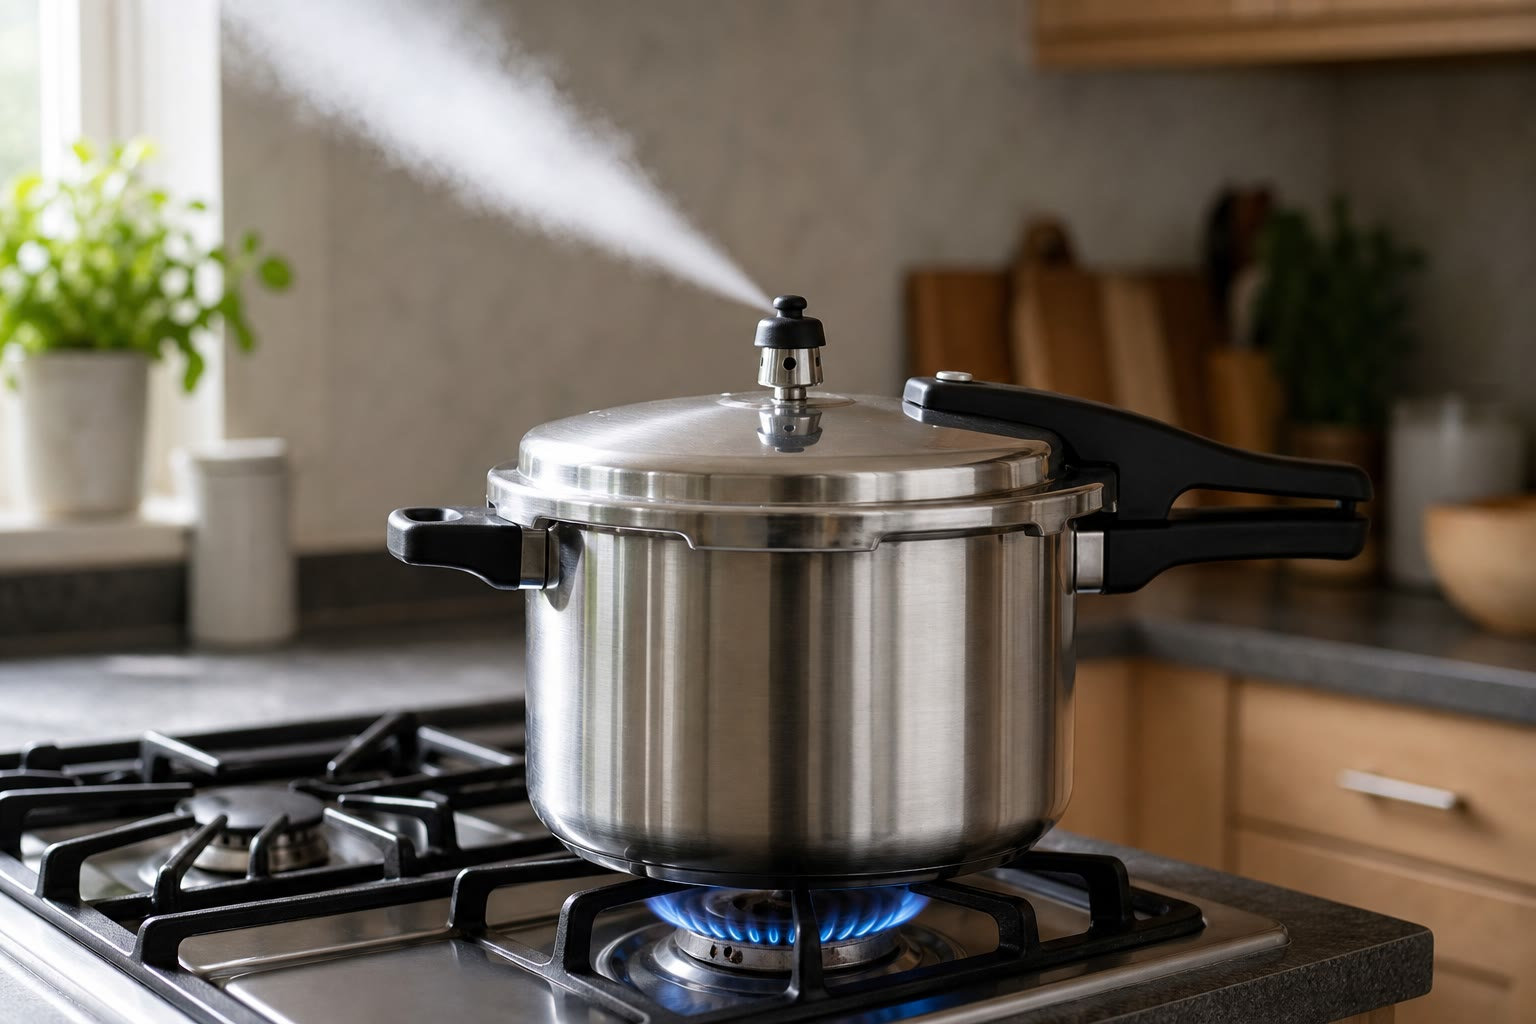
\includegraphics[width=0.58\linewidth]{images/book3/ai/b3-25-pressure-cooker-steam.jpg}

{\small Una olla a presión: a \qty{1.8}{bar} el agua hierve a \qty{117}{\degreeCelsius}, y es la válvula lastrada la que fija la presión.}
\end{omfigure}

\section{Problema: el agua en cuatro escenas}

\begin{problem}[{Problema de fin de semana --- la olla a presión, la nube,
el recipiente cerrado y la botella en sobrefusión: un solo cuerpo, cuatro
usos de su diagrama de fases}]
\label{pb:b1:phase-changes:1}
Datos del agua: $L_v = \qty{2257}{kJ/kg}$ a \qty{100}{\degreeCelsius} y
alrededor de \qty{2.2}{MJ/kg} a \qty{117}{\degreeCelsius}, \qty{2.45}{MJ/kg} cerca de
\qty{20}{\degreeCelsius}; $L_f = \qty{334}{kJ/kg}$; $c = \qty{4.18}{kJ/(kg.K)}$
(líquido); $M = \qty{18}{g/mol}$; $ML_v/R = \qty{4890}{K}$ cerca de
\qty{100}{\degreeCelsius}. Presiones de saturación: \qty{0.61}{kPa}
(\qty{0}{\degreeCelsius}), \qty{1.23}{kPa} (\qty{10}{\degreeCelsius}), \qty{1.70}{kPa} (\qty{15}{\degreeCelsius}),
\qty{2.34}{kPa} (\qty{20}{\degreeCelsius}), \qty{3.17}{kPa} (\qty{25}{\degreeCelsius}), \qty{4.24}{kPa}
(\qty{30}{\degreeCelsius}), \qty{101.3}{kPa} (\qty{100}{\degreeCelsius}).
Volúmenes másicos saturantes: $v_l = \qty{1.0e-3}{m^3/kg}$ (agua fría) y
\qty{1.9e-3}{m^3/kg} a \qty{360}{\degreeCelsius}; $v_v = \qty{0.0217}{m^3/kg}$
a \qty{300}{\degreeCelsius}, $0.0108$ a \qty{340}{\degreeCelsius} y $0.0088$
a \qty{350}{\degreeCelsius}; \omterm{prop:b1:phase-changes:PTdiagram}{punto crítico} \qty{374}{\degreeCelsius},
\qty{221}{bar}, $v_c = \qty{3.1e-3}{m^3/kg}$. Aire: $M = \qty{29}{g/mol}$, $c_p =
\qty{1.0}{kJ/(kg.K)}$, $\gamma = 1.4$; $g = \qty{9.8}{m/s^2}$; $R =
\qty{8.314}{J/(mol.K)}$.

\medskip
\noindent\textbf{Parte I --- La olla a presión.}
\begin{enumerate}
  \item ¿Por qué no puede calentarse por encima de \qty{100}{\degreeCelsius}
        el agua de una cazuela abierta a nivel del mar, por fuerte que sea
        la llama?
  \item A partir de la \omterm{thm:b1:phase-changes:clapeyron}{relación de Clausius--Clapeyron}, dedúzcase
        $\ln[P_s(T)/P_s(T_0)] = (ML_v/R)(1/T_0 - 1/T)$, enunciando las
        aproximaciones.
  \item Temperatura en una olla cuya válvula abre a \qty{1.8}{bar}
        absolutos.
  \item La válvula es una pesa apoyada sobre un orificio de \qty{20}{mm^2};
        presión atmosférica \qty{1.0}{bar}: masa de la pesa.
  \item \qty{2.0}{L} de agua se llevan de \qty{20}{\degreeCelsius} a la
        temperatura de trabajo con una placa de \qty{2.0}{kW}
        (despréciese la olla): calor y tiempo.
  \item Una vez allí, se deja la placa a \qty{2.0}{kW}: masa de vapor que
        sale por la válvula cada minuto. ¿Qué debería hacer el cocinero?
  \item Las reacciones de la cocción duplican aproximadamente su velocidad
        cada \qty{10}{K}: ¿en qué factor acorta la olla una receta de
        \qty{30}{min} a nivel del mar? ¿Y cuánto duraría esa receta en el
        Everest, donde el agua hierve a \qty{70}{\degreeCelsius}?
\end{enumerate}

\medskip
\noindent\textbf{Parte II --- La nube.}
\begin{enumerate}[resume]
  \item Defínase la \omterm{ex:b1:phase-changes:dew}{humedad relativa}. Aire a \qty{25}{\degreeCelsius} y $60\%$:
        presión parcial del vapor y masa de vapor por metro cúbico
        (\omterm{def:b1:kinetic-theory:model}{gas perfecto}).
  \item \omterm{ex:b1:phase-changes:dew}{Punto de rocío} de ese aire (interpólese la tabla). Explíquense el
        rocío sobre la hierba al alba y las gotas en una botella fría.
  \item Una parcela de aire seco asciende sin intercambiar calor. A partir
        de la ley adiabática reversible y de la relación de la estática de
        fluidos $\dd P/\dd z = -\rho g$, muéstrese que $\dd T/\dd z = -g/c_p$ y
        evalúese.
  \item El \omterm{ex:b1:phase-changes:dew}{punto de rocío} de la parcela ascendente baja a su vez unos
        \qty{2}{K/km} al caer la presión. Altura a la que la parcela de la
        pregunta~8 queda saturada --- la base de la nube.
  \item Por encima de la base, el vapor que condensa libera su \omterm{def:b1:phase-changes:phase}{calor
        latente} en la parcela. ¿En cuánto calienta ese aire la
        condensación de \qty{1}{g} de agua por kilogramo de aire? ¿Qué
        hace eso con el ritmo de enfriamiento de la parcela mientras sigue
        subiendo, y por qué importa para las tormentas?
  \item Un cúmulo de \qty{1}{km^3} contiene \qty{1}{g} de agua líquida por
        metro cúbico: masa de agua y energía que libera su condensación,
        en julios y en \unit{GW h}.
  \item Un espejo de baño a \qty{18}{\degreeCelsius}, con el aire a
        \qty{25}{\degreeCelsius} y un $80\%$: ¿se empaña? ¿Con qué humedad
        dejaría de hacerlo?
\end{enumerate}

\medskip
\noindent\textbf{Parte III --- El recipiente cerrado.}
Un recipiente rígido de acero de \qty{1.0}{L} se llena con una masa $m$ de
agua y se cierra sin aire; después se calienta lentamente.
\begin{enumerate}[resume]
  \item $m = \qty{0.50}{kg}$ a \qty{20}{\degreeCelsius}: presión interior,
        volumen másico, masa de vapor (úsese el \omterm{def:b1:kinetic-theory:model}{gas perfecto} para $v_v$) y
        fracción del volumen ocupada por el líquido.
  \item Al calentarlo, ¿sube o baja el nivel del líquido? ¿A qué
        temperatura, aproximadamente, llena el líquido el recipiente, y
        qué le ocurre después a la presión? (Úsese $v_l$ a \qty{360}{\degreeCelsius}.)
  \item $m = \qty{0.10}{kg}$: ¿sube o baja el nivel del líquido al
        calentar? ¿A qué temperatura, aproximadamente, se evapora la
        última gota (úsese la tabla de $v_v$)?
  \item $m = \qty{0.31}{kg}$: descríbase lo que ve un observador en el
        menisco cuando la temperatura se acerca a \qty{374}{\degreeCelsius}.
  \item Dibújense los tres caminos de calentamiento en el diagrama
        $(v, P)$ con la campana de saturación, y dígase por qué lado del
        \omterm{prop:b1:phase-changes:PTdiagram}{punto crítico} pasa cada uno.
  \item El mismo recipiente de \qty{1.0}{L} con \qty{0.50}{kg} de agua se
        cierra ahora \emph{con} el aire que contenía a \qty{20}{\degreeCelsius}
        y \qty{1.0}{bar}, y se calienta hasta \qty{100}{\degreeCelsius}:
        presión total interior (Dalton) y fuerza sobre una tapa de \qty{100}{cm^2}.
\end{enumerate}

\medskip
\noindent\textbf{Parte IV --- La botella en \omterm{def:b1:phase-changes:metastable}{sobrefusión}.}
\begin{enumerate}[resume]
  \item Una botella de agua limpia y en reposo se ha enfriado hasta
        \qty{-8}{\degreeCelsius} sin congelarse. ¿Cómo se llama este estado,
        por qué es posible y qué ocurre al golpear la botella? ¿Por qué se
        queda entonces la temperatura exactamente en \qty{0}{\degreeCelsius}?
  \item Fracción del agua que se congela (el proceso es rápido, luego
        adiabático).
  \item Entropía creada por kilogramo; compruébese el signo.
  \item La sorpresa contraria: una taza de agua calentada a \qty{105}{\degreeCelsius}
        en un horno microondas sin hervir, y luego perturbada. Fracción
        del agua que se convierte de golpe en vapor, volumen de vapor
        producido por litro ($v_v = \qty{1.67}{m^3/kg}$) y por qué estalla la taza.
  \item \omterm{thm:b1:heat-engines:lostwork}{Trabajo perdido}: el litro en \omterm{def:b1:phase-changes:metastable}{sobrefusión} podría haber accionado
        una máquina reversible con el entorno a \qty{0}{\degreeCelsius};
        tomando $T_0 = \qty{273}{K}$, el trabajo que se tira al dejarlo
        congelarse de un golpe vale $T_0S_{\mathrm{created}}$. Evalúese por
        litro y compárese con subir la botella un metro. Conclúyase: ¿qué
        almacena un \omterm{def:b1:phase-changes:metastable}{estado metaestable}?
\end{enumerate}
\end{problem}
